\documentclass{article}%
\usepackage[T1]{fontenc}%
\usepackage[utf8]{inputenc}%
\usepackage{lmodern}%
\usepackage{textcomp}%
\usepackage{lastpage}%
\usepackage{authblk}%
\usepackage{graphicx}%
%
\title{Epigenetic Regulation of Cardiac Progenitor Cells Marker c{-}kit by Stromal Cell Derived Factor{-}1a}%
\author{Janice Williams}%
\affil{Institute of Orthopedic Surgery, Xijing Hospital, Fourth Military Medical University, Xian, Peoples Republic of China}%
\date{01{-}01{-}2014}%
%
\begin{document}%
\normalsize%
\maketitle%
\section{Abstract}%
\label{sec:Abstract}%
(SOURCE: GTF International)\newline%
By Dr. Lucas Hedges\newline%
The research, presented today at the International Society for Stem Cell Research (ISSCR) 2013, shows a tina stimulates the cell growth of the vascular smooth muscle cells and the tina results in structural consolidation, which improves elasticity and skin improvement.\newline%
The research has also discovered an unexpected dietary effect which could benefit patients with patients with high blood pressure and high cholesterol and could also help prevent the release of cholesterol.\newline%
The study is published in the current issue of the ISSCR, and on a consortium level with all 50 key conferences within the ISSCR 2013 {-} the worlds largest event of its kind.\newline%
Stem cell specialists at the University of California, San Diego School of Medicine reviewed every step of the research which involved the scientists and researchers at the University of Texas Medical Branch in Galveston.\newline%
Head of the Multi{-}Ethnic Stem Cell/Stem Cell Development Group at UCSDs Discovery Institute, Dr. Lucas Hedges, said, This research shows a fascinating chemical effect that can benefit both patients with vascular diseases and people with other diseases.\newline%
The bioactive bioactive products we found in this study were created as a quid pro quo with cells which are genetically produced by the patient and fed to another cell from the patients own body, thus encouraging cells to form a special form that creates a protective barrier around skin and has a decreased elasticity.\newline%
This clearly provides new insights about how the patient develops a healthy, long{-}term immune response to it and potentially changes outcomes in the patient with vascular disease, to the degree that traditional cell therapy cant achieve these goals.\newline%
Dr. Hedges added that the ability to regulate abnormal immune responses to endothelial cells in the blood is one of the most important advances in understanding how human cells function.\newline%
The complex cell pathologist continues to study the molecular mechanisms through which cell death plays a role in the progression of vascular disease and to develop novel treatments.\newline%
Dr. Hedges adds, One of the main goals in these experiments is to show that gene therapy from an unrelated patient can be effective and safe.\newline%
The study, which is being presented this morning at the ISTC 2013, shows that genes were elevated and in some cases inhibited to a degree in a population of individuals which is considered sufficiently small in number to be innovative.\newline%
Those increases in genes can contribute to potentially debilitating outcomes in patients, which may be prevented by discovering and ultimately curing a disease.

%
\subsection{Image Analysis}%
\label{subsec:ImageAnalysis}%


\begin{figure}[h!]%
\centering%
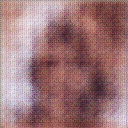
\includegraphics[width=150px]{500_fake_images/samples_5_315.png}%
\caption{A Close Up Of A Cat In A Mirror}%
\end{figure}

%
\end{document}